\documentclass[12pt,a4paper,oneside]{book}
\input{config.tex}

\title{Ingegneria del Software}
\author{Michela Maria Tasca \\ \small Prof. Calvagna --- UniCt}
\date{A.A. 2025/2026}

\begin{document}

\maketitle
\tableofcontents

\chapter{Introduzione all'Ingegneria del Software}

\section{Il Problema: Perché l'Ingegneria del Software?}

Nello sviluppo del software, l'assenza di principi ingegneristici porta a fallimenti visibili e costosi. Un esempio classico è l'immagine di un \textbf{billboard del mago Lance Burton, interrotto da una finestra di dialogo di errore di Windows} . 
\begin{figure}[H]
    \centering
    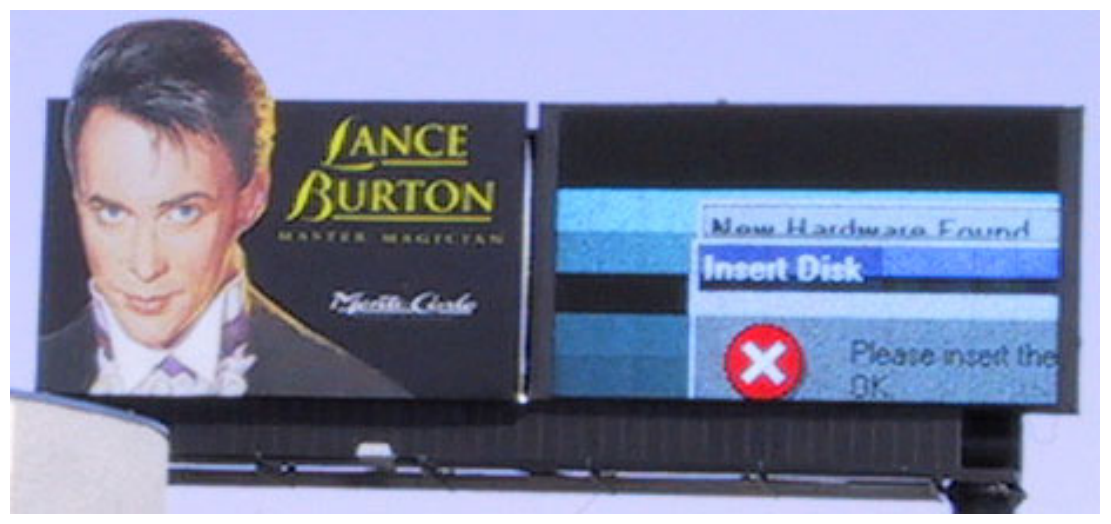
\includegraphics[width=0.8\textwidth]{cartellone.png}
    \label{fig:nome_riferimento}
\end{figure}

Questo errore nel mondo reale evidenzia un difetto critico nella progettazione dei sistemi embedded o di produzione. In un ambiente di produzione, un sistema software non deve mai esporre dettagli di basso livello o bloccare l'esecuzione per attendere l'input di un utente inesistente. Questo fallimento sottolinea l'importanza della \textbf{robustezza}, della gestione corretta delle eccezioni e della configurazione adeguata dell'ambiente di sviluppo, concetti cardine dell'Ingegneria del Software per garantire la \textit{dependability} del sistema.

Altri fallimenti storici dovuti a bug software includono:
\begin{itemize}
    \item \textbf{Mars Climate Orbiter (1999):} Perso a causa di un errore di riuso dei componenti (mancata conversione tra sistema metrico decimale e imperiale).
    \item \textbf{Mars Polar Lander (1999):} Fallito per una violazione delle precondizioni nel software.
    \item \textbf{USS Yorktown (1997):} L'incrociatore è rimasto bloccato in mare per ore a causa di un'eccezione non gestita (divisione per zero) inserita da un operatore, che ha causato un buffer overflow.
    \item \textbf{Space Shuttle Columbia:} Il primo lancio fu ritardato per un problema di sincronizzazione causato dalla modifica di un fattore di ritardo da 50 a 80 millisecondi anni prima.
\end{itemize}

\section{Definizione e Storia}

Il termine \textit{Software Engineering} è nato nel 1968 durante la Conferenza NATO di Garmisch, per rispondere alla "crisi del software": i progetti non rispettavano le scadenze, superavano i budget e producevano software di bassa qualità.

Una figura chiave è stata \textbf{Margaret Hamilton}, ritratta accanto a una \textbf{pila di codici stampati su carta alta quanto lei}.
\begin{figure}[H]
    \centering
    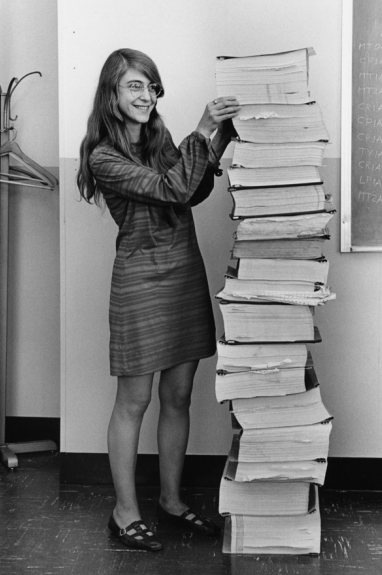
\includegraphics[width=0.5\linewidth]{image.png}
    \label{fig:placeholder}
\end{figure}
La foto mostra il codice sorgente del software di volo delle missioni Apollo (Apollo Guidance Computer). La Hamilton ha coniato il termine "Ingegneria del Software" lottando affinché lo sviluppo del codice ricevesse lo stesso rispetto, legittimità e rigore metodologico riservato all'hardware, permettendo all'umanità di arrivare sulla Luna senza crash di sistema critici.

\begin{definition}{Ingegneria del Software (Definizione Preliminare)}{}
La disciplina che studia il processo di costruzione di un prodotto software.
\end{definition}

Per comprendere la portata di questa disciplina, bisogna considerare la dimensione tipica dei prodotti software, il numero di persone necessarie per costruirli, e l'impatto critico di eventuali ritardi o bug (che possono costare vite umane o miliardi di dollari, come nel caso del \textbf{Space Shuttle Software}, che superò il budget di 10 miliardi di dollari ed ebbe 3 anni di ritardo per un errore di sincronizzazione).

\begin{definition}{Ingegneria del Software (Definizione Completa)}{}
L'Ingegneria del Software è un insieme di tecniche, metodologie e strumenti che aiutano nella produzione di un sistema software di \textbf{alta qualità}, rispettando un \textbf{budget} e una \textbf{scadenza} prefissati, gestendo al contempo il \textbf{cambiamento} continuo dei requisiti.
\end{definition}

\section{Il Processo di Sviluppo Software}

\begin{definition}{Processo Software}{}
Un insieme di attività e le relative relazioni che supportano lo sviluppo o l'evoluzione di un sistema software. Risponde a domande su quali attività selezionare, le loro dipendenze e la loro pianificazione.
\end{definition}

Le attività generiche in tutti i processi software sono:
\begin{itemize}
    \item \textbf{Analisi e Specifica:} Definire cosa deve fare il sistema e i suoi vincoli.
    \item \textbf{Sviluppo (Development):} La produzione vera e propria del codice.
    \item \textbf{Validazione:} Verificare che il software corrisponda a ciò che il cliente desidera.
    \item \textbf{Manutenzione / Evoluzione:} Modificare il software in risposta a nuove richieste.
\end{itemize}
\newpage
\subsection{Modelli di Processo (Analisi dei Diagrammi)}

\subsubsection{Il Modello a Cascata (Waterfall Model)}
\begin{figure}[H]
    \centering
    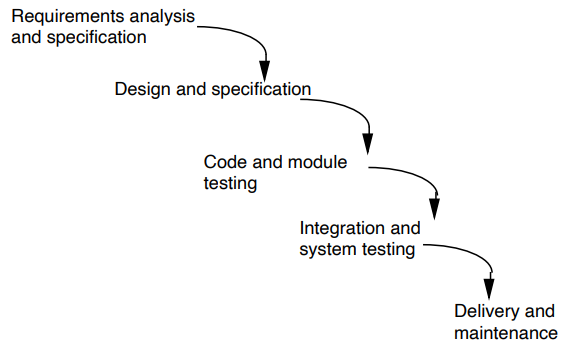
\includegraphics[width=0.5\linewidth]{waterfall.png}
    \label{fig:placeholder}
\end{figure}
Il diagramma del ciclo di vita classico mostra un flusso sequenziale in cui ogni fase produce gli artefatti necessari per la successiva:
\begin{enumerate}
    \item \textbf{Requirements analysis and specification} (Analisi dei requisiti).
    \item \textbf{Design and specification} (Progettazione).
    \item \textbf{Code and module testing} (Implementazione e test di unità).
    \item \textbf{Integration and system testing} (Integrazione e collaudo).
    \item \textbf{Delivery and maintenance} (Rilascio e manutenzione).
\end{enumerate}

\subsubsection{Il Processo di Sviluppo (Enhanced Model)}
\begin{figure}[H]
    \centering
    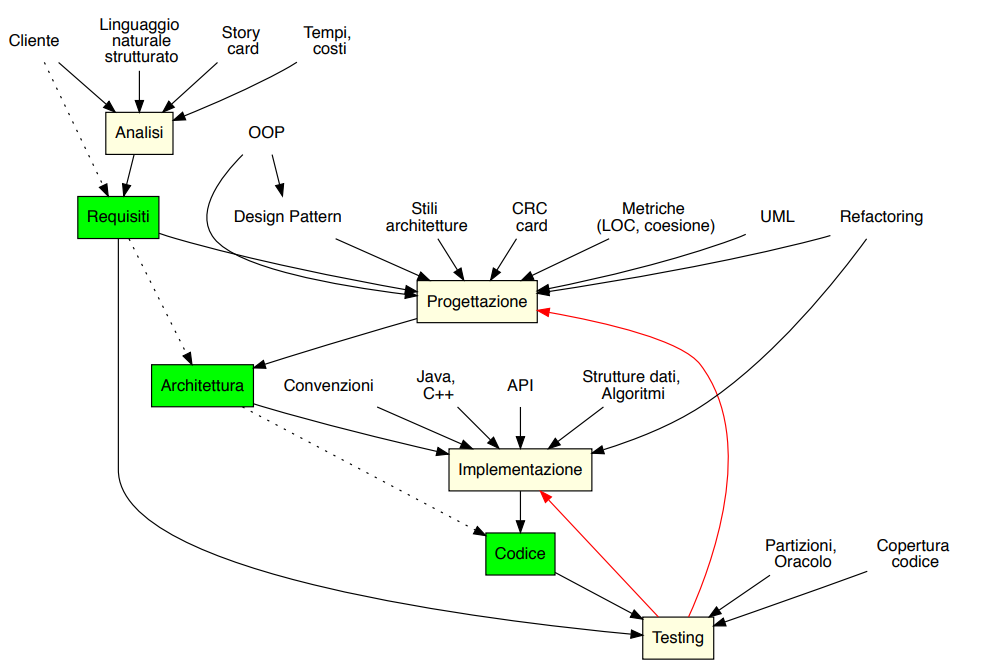
\includegraphics[width=0.75\linewidth]{imm.png}
    \label{fig:placeholder}
\end{figure}
Il diagramma del modello esteso illustra un approccio più iterativo e basato su concetti moderni:
\begin{itemize}
    \item \textbf{Attori e Input:} Il \textit{Cliente} fornisce requisiti sotto forma di \textit{Linguaggio naturale strutturato}, \textit{Story card} o \textit{Use case}.
    \item \textbf{Fase di Analisi:} Produce i documenti di specifica.
    \item \textbf{Fase di Progettazione:} Riceve input dall'analisi e applica concetti come \textit{OOP, Design Pattern, Architetture software e CRC card}.
    \item \textbf{Fase di Implementazione:} Traduce il design in codice utilizzando \textit{Convenzioni, API, Strutture dati e Algoritmi}.
    \item \textbf{Fase di Testing:} Utilizza artefatti come \textit{Partizioni, Oracoli e Copertura del codice} per validare il prodotto, con un ciclo di feedback (\textit{Refactoring} e \textit{UML}) che torna verso la progettazione e l'implementazione.
\end{itemize}

\section{Forze Guida (Drivers) e Ruolo dell'Ingegnere}

Il processo e il prodotto sono influenzati da diverse forze (Drivers) interconnesse:
\begin{figure}[H]
    \centering
    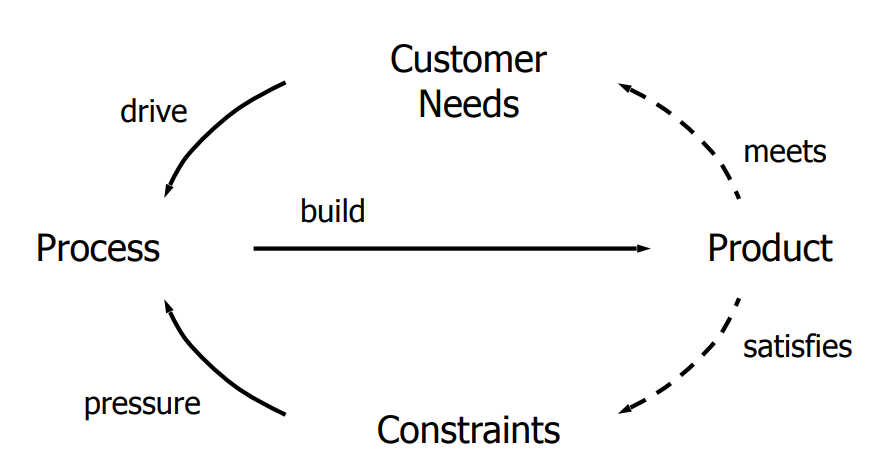
\includegraphics[width=0.5\linewidth]{process.png}
    \label{fig:placeholder}
\end{figure}
\begin{itemize}
    \item \textbf{Customer Needs (Requisiti dei clienti/utenti):} Guidano il processo.
    \item \textbf{Process (Team e Processi):} Costruiscono il prodotto.
    \item \textbf{Product (Tecnologia):} Soddisfa i vincoli e le necessità.
    \item \textbf{Constraints (Contesto, Leggi, Budget):} Esercitano pressione sul processo.
\end{itemize}
Un cambiamento significativo in una di queste forze (es. passare da 10 rilasci al giorno a 1 rilascio ogni 100 giorni per motivi normativi) altera l'intera architettura e struttura del team.
Come suggerito da \textbf{Jeff Dean} (Google), una variazione di \textbf{10x} nelle dimensioni di un progetto rende le vecchie soluzioni sub-ottimali, mentre una variazione di \textbf{100x} richiede approcci e strutture organizzative radicalmente nuove.

\subsection{Scienziato vs Ingegnere del Software}
\begin{itemize}
    \item \textbf{Computer Scientist:} Dimostra teoremi, definisce linguaggi, lavora senza vincoli di tempo stringenti.
    \item \textbf{Software Engineer:} Lavora in domini applicativi multipli, deve risolvere i problemi del cliente in tempi ridotti (es. 3 mesi), integrando strumenti e metodologie mentre i requisiti e le tecnologie cambiano. Richiede forti doti comunicative, di astrazione, di modellazione e capacità di lavorare in team.
\end{itemize}

\section{La Qualità del Software}
La valutazione del software si basa su criteri operativi:
\begin{itemize}
    \item \textbf{Correttezza:} Il software fa ciò che il cliente vuole? (\textit{Validazione funzionale}). Soddisfa le specifiche tecniche? (\textit{Verifica tecnica}).
    \item \textbf{Efficienza, Dependability (Sicurezza/Affidabilità), Usabilità.}
    \item \textbf{Manutenibilità (Maintainability):} È il criterio più critico e costoso. Poiché il software non ha parti fisiche, è intrinsecamente modificabile. Se un software ha successo, sopravviverà all'hardware originale e dovrà inevitabilmente evolvere per adattarsi a nuovi requisiti.
\end{itemize}

\section{Le Sfide Fondamentali in Ingegneria del Software}
Le tre sfide principali che gli ingegneri devono affrontare sono: \textbf{Cambiamento}, \textbf{Complessità} e \textbf{Difetti}.

\subsection{1. I Requisiti Cambiano}
I requisiti degli utenti (bisogni, obiettivi) mutano nel tempo. Il fallimento di un prodotto nel soddisfare l'utente, pur avendo seguito le specifiche iniziali, impone di adottare un \textbf{Processo} flessibile in grado di assorbire i cambiamenti.

\subsection{2. Il Software è intrinsecamente Complesso}
Il software è complesso perché è difficile da comprendere e modificare.
\begin{definition}{Complessità Accidentale vs Complessità Intrinseca}{}
\textbf{Complessità Accidentale:} È legata a scelte di implementazione inadeguate. Può essere rimossa pulendo il codice (refactoring), cambiando linguaggio o ripagando il \textit{Debito Tecnico}.\\
\textbf{Complessità Intrinseca:} Rimane anche dopo aver rimosso l'accidentale. Deriva dal fatto che il comportamento a \textit{run-time} (dinamico) è invisibile rispetto al testo statico del codice sorgente.
\end{definition}

L'imprevedibilità del comportamento dinamico rende impossibile anticipare tutti gli stati del programma. Per gestire la complessità intrinseca, è necessario applicare \textbf{Design Pattern}, progettare sistemi modulari, mantenere un \textbf{basso accoppiamento} (low coupling) e un'\textbf{alta coesione} (high cohesion).

\textbf{Esempio di Complessità Intrinseca:}
Dato il seguente frammento di codice la domanda è: il loop finisce?

\begin{lstlisting}[language=Java]
do j++;
    while a[j] >= pivot;
\end{lstlisting}
La risposta dipende dal valore di \texttt{j}, di \texttt{pivot}, e dell'elemento dell'array. La conclusione è che lo stesso codice potrebbe, potenzialmente avere infiniti outcome.

\subsection{3. I Difetti sono Inevitabili}
Come dimostrato dagli esperimenti di \textbf{George Miller} (anni '50), la mente umana può gestire simultaneamente circa 7 blocchi di informazioni (\textit{chunks}). Oltre questa soglia, insorgono confusione ed errori. Poiché il software supera facilmente questa soglia, per garantire la qualità bisogna \textbf{Testare (Validare)} o \textbf{Dimostrare (Verificare)} la correttezza del prodotto.

\begin{definition}{Fault (Difetto) vs Failure (Fallimento)}{}
\textbf{Fault (Difetto o Bug):} È un'anomalia statica presente nel codice sorgente o nei documenti di specifica.\\
\textbf{Failure (Fallimento):} È il comportamento anomalo scatenato a \textit{run-time} (dinamicamente) da un Fault. Ad esempio, un'app che va in \textit{crash} subisce un failure; il failure si manifesta solo in determinate condizioni, ma il fault è sempre presente nel codice.
\end{definition}

\chapter{Da C++ a Java}
\section{Origini e Caratteristiche di Java}
Java è stato sviluppato nei primi anni '90 da un team della Sun Microsystems guidato da James Gosling.
\begin{itemize}
    \item Originariamente chiamato \textbf{Oak} (ispirato a un albero fuori dall'ufficio di Gosling).
    \item Inizialmente pensato per la programmazione di smart TV e altri dispositivi, è stato rapidamente riadattato per il Web emergente (prima release nel 1995).
    \item È uno dei linguaggi più popolari al mondo, ampiamente usato nello sviluppo di software enterprise.
    \item Possiede una vasta libreria di funzionalità integrate, garantisce buone prestazioni ed elevata portabilità.
    \item È il linguaggio predefinito per i dispositivi mobili Android e per giochi come Minecraft.
    \item Appartiene alla famiglia dei linguaggi \textbf{Object-Oriented (OO)}: i programmi sono organizzati in unità chiamate classi e oggetti.
\end{itemize}

\section{Ambiente di Esecuzione: C++ vs Java}
Di seguito due schemi che mettono a confronto i processi di compilazione ed esecuzione tra C++ e Java. Questo confronto è cruciale per comprendere le differenze di portabilità e performance.

\begin{figure}[H]
    \centering
    \begin{subfigure}[b]{0.45\textwidth}
        \centering
        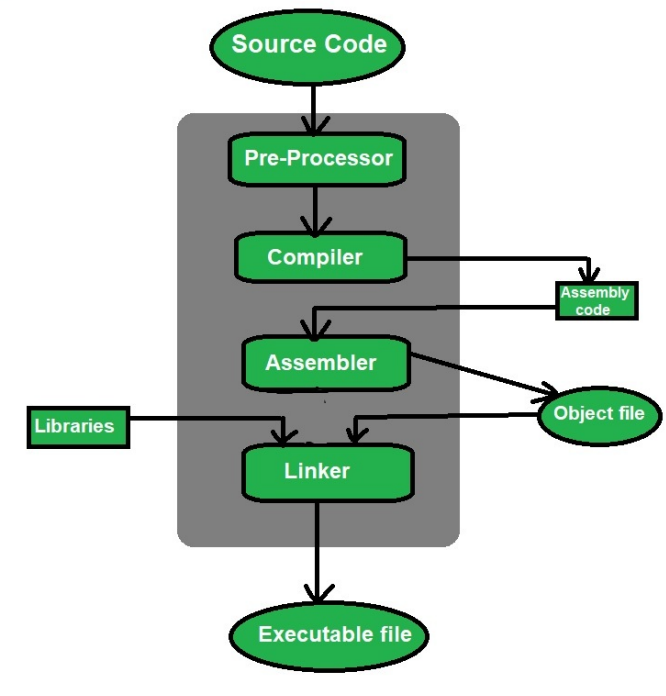
\includegraphics[width=\textwidth]{esecuzioneC.png}
        \caption{C/C++ Program Environment}
        \label{fig:img_C}
    \end{subfigure}
    \hfill
    \begin{subfigure}[b]{0.45\textwidth}
        \centering
        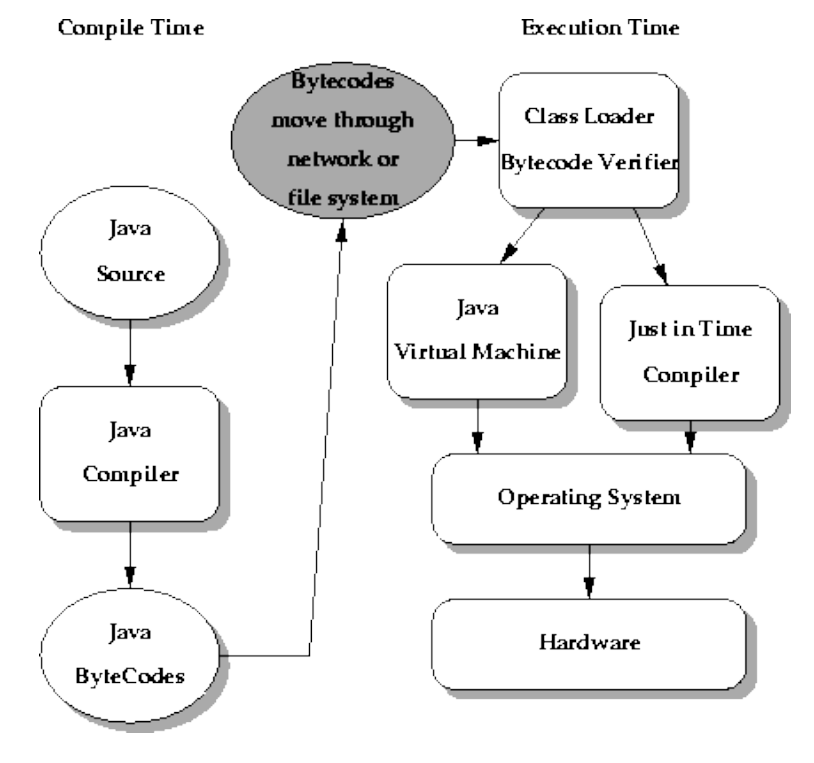
\includegraphics[width=\textwidth]{esecuzionejava.png}
        \caption{Java Program Environment}
        \label{fig:img_J}
    \end{subfigure}
    \label{fig:esecuzioni}
\end{figure}

Il primo diagramma, che si riferisce all'esecuzione del codice in C/C++ mostra un processo di compilazione nativa diretta:
\begin{enumerate}
    \item \textbf{Source Code:} Il codice sorgente passa al \textbf{Pre-Processor}.
    \item \textbf{Compiler:} Il codice pre-processato viene tradotto in assembly.
    \item \textbf{Assembler:} Genera l'\textbf{Object File}.
    \item \textbf{Linker:} Collega le librerie esterne e genera l'\textbf{Executable File}.
    \item L'eseguibile viene poi eseguito direttamente sull'hardware. Questo lo rende veloce ma dipendente dalla piattaforma (non portabile).
\end{enumerate}

Il diagramma per Java mostra invece un approccio ibrido (compilazione + interpretazione):
\begin{enumerate}
    \item \textbf{Compile Time:} Il \textbf{Java Source} viene processato dal \textbf{Java Compiler}, che genera i \textbf{Bytecodes}. Questi bytecodes possono viaggiare attraverso la rete o il file system.
    \item \textbf{Execution Time:} Il \textbf{Class Loader} e il \textbf{Bytecode Verifier} caricano il bytecode nella \textbf{Java Virtual Machine (JVM)}.
    \item La JVM utilizza un \textbf{Just in Time (JIT) Compiler} per tradurre il bytecode in istruzioni macchina specifiche per l'\textbf{Operating System} e l'\textbf{Hardware} sottostante. Questo garantisce la portabilità ("Write Once, Run Anywhere").
\end{enumerate}

\section{Differenze Architetturali: C++ vs Java}
Il confronto tra C++ e Java evidenzia filosofie di design profondamente diverse, specialmente nella gestione della memoria e nell'Object Orientation.
\begin{itemize}
    \item \textbf{Paradigma OOP Puro:} In Java tutto deve risiedere all'interno di una classe (o interfaccia). \textbf{Non esistono variabili globali} libere. Una variabile \texttt{public static} simula il concetto di variabile globale, ma resta confinata in un namespace di classe.
    \item \textbf{Tipizzazione Fortemente Controllata (Strong Type Checking):} Come il C++, i tipi devono essere compatibili a tempo di compilazione. Java aggiunge un rigoroso controllo sul \textbf{tipo dinamico} a runtime: un identificatore (reference) può puntare a oggetti di classi derivate, ma l'effettivo uso deve rispettare le gerarchie di ereditarietà.
    \item \textbf{Ereditarietà:} Java \textbf{non supporta l'ereditarietà multipla} tra classi per evitare il "Problema del diamante" (ambiguità nella risoluzione dei metodi). Questo design limitante è aggirato dal supporto all'implementazione di interfacce multiple.
    \item \textbf{Radice della Gerarchia:} Tutte le classi Java derivano implicitamente dalla superclasse \textbf{\texttt{Object}}.
    \item \textbf{Puntatori e Identificatori:} In Java gli identificatori a tipi non primitivi \textbf{sono di fatto puntatori} (reference), ma non è consentita l'aritmetica dei puntatori (es. \texttt{b++} è illegale). L'operatore \texttt{.} sostituisce l'uso di \texttt{->} del C++.
    \item \textbf{Gestione della Memoria:} A differenza del C++ dove la memoria allocata dinamicamente con \texttt{new} richiede una \texttt{delete} esplicita, in Java la deallocazione è delegata al \textbf{Garbage Collector}, che interviene automaticamente per eliminare gli oggetti non più referenziati, prevenendo i memory leak.
\end{itemize}

\begin{itemize}
    \item Il significato del separatore punto (\texttt{.}) in Java è lo stesso dell'operatore freccia (\texttt{->}) in C++.
    \item \textbf{Gli identificatori in Java sono tutti puntatori} (riferimenti agli oggetti).
    \item Non ci sono entità esterne agli oggetti: nulla può essere definito al di fuori di un costrutto di classe o interfaccia. Di conseguenza, \textbf{non esistono variabili globali} (anche se una classe con un attributo statico funge da pseudo-globale).
    \item Non serve il punto e virgola (\texttt{;}) alla fine dei blocchi dichiarativi delle classi \texttt{\{\}}.
    \item In una classe vengono inserite contestualmente sia l'astrazione (l'Abstract Data Type, ADT) che la sua implementazione.
    \item Java è \textbf{fortemente tipizzato (strong type checking)} come il C++. I tipi ai lati di un assegnamento devono essere formalmente compatibili a tempo di compilazione.
    \item Java esegue anche un controllo sul \textbf{tipo dinamico}: un identificatore può puntare a oggetti di tipo diverso in momenti diversi dell'esecuzione, ma il tipo effettivo a runtime deve sempre essere compatibile con il tipo a cui lo si assegna.
    \item Java \textbf{non supporta l'ereditarietà multipla} per evitare il "Problema del diamante". Questo comportamento è però replicabile tramite l'uso delle \textbf{interfacce}.
    \item La radice della gerarchia delle classi in Java è unica ed è la classe \textbf{Object}.
    \item La libreria standard si trova nel dominio \texttt{java.*}.
    \item È consentita una sola classe pubblica per file (salvo classi nidificate) e il file deve avere lo stesso nome della classe.
    \item Il metodo \texttt{main} deve obbligatoriamente essere definito all'interno di una classe.
    \item L'istruzione \texttt{import} (a differenza degli \texttt{\#include} in C++ che importano interi file header) indica gruppi di librerie o singole classi per nome composto.
\end{itemize}

\section{Identificatori e Puntatori}
\begin{itemize}
    \item \textbf{In C++:} L'istruzione \texttt{T a;} alloca direttamente una struct/oggetto \texttt{T}. L'istruzione \texttt{T *b = new T();} alloca dinamicamente un puntatore e richiede l'uso esplicito di \texttt{delete(b)} per deallocare la memoria. È consentita l'aritmetica dei puntatori (es. \texttt{b++}). L'accesso ai membri avviene tramite \texttt{a.m()} o \texttt{b->m()}.
    \item \textbf{In Java:} L'istruzione \texttt{T a;} dichiara solo un identificatore (riferimento), ma non alloca l'oggetto. L'istruzione \texttt{T a = new T();} alloca dinamicamente l'istanza. L'aritmetica dei puntatori è \textbf{illegale}. L'assegnamento tra oggetti (\texttt{a = b}) copia il riferimento, non l'oggetto in sé. La deallocazione della memoria è gestita automaticamente dal \textbf{Garbage Collector}. L'accesso ai membri avviene \textbf{sempre e solo} col punto (\texttt{a.m()}).
\end{itemize}

\section{Metodi e Override}
La gestione del dispatching dei metodi (risoluzione delle chiamate a metodo) varia tra i due linguaggi:
\begin{itemize}
    \item \textbf{Java:} Il dispatch è a \textbf{run-time} ed è \textbf{automatico}. Non è necessaria alcuna keyword per l'override. I metodi non virtuali (che non possono subire override) sono quelli contrassegnati come \texttt{final}, \texttt{static} o \texttt{private}.
    \item \textbf{C++:} Il dispatch avviene a run-time \textbf{solo se} è presente la keyword \texttt{virtual}. Di default, i metodi sono non virtuali e non richiedono keyword specifiche.
\end{itemize}

\section{Esempio Pratico: Hello World e Diagramma UML}
Nelle slide viene analizzato il classico esempio "Hello World" con l'ausilio di un Class Diagram UML, fondamentale in Ingegneria del Software per modellare la struttura statica del sistema.

\subsection{Analisi del Class Diagram UML}
Nella progettazione software, i Class Diagram UML modellano la \textbf{struttura statica} di un sistema, definendo le entità, i loro attributi (stato) e metodi (comportamento). Di seguito il diagramma UML della classe \texttt{HelloWorld}:
\begin{figure}[H]
    \centering
    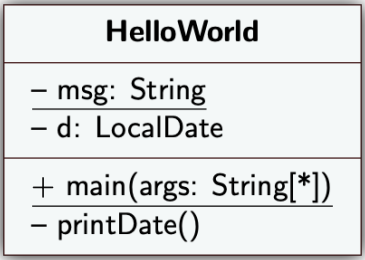
\includegraphics[width=0.35\linewidth]{Hello.png}
    \caption{"Hello World" UML Diagram}
    \label{fig:placeholder}
\end{figure}
Il diagramma UML rappresenta la classe \texttt{HelloWorld} con la seguente struttura formale:
\begin{itemize}
    \item \textbf{Nome Classe:} \texttt{HelloWorld}
    \item \textbf{Attributi (Fields):}
    \begin{itemize}
        \item \texttt{- msg: String}: La visibilità privata (\texttt{-}) impone l'incapsulamento. Il campo è di tipo String.
        \item \texttt{- d: LocalDate}: Variabile privata per conservare un'istanza temporale.
    \end{itemize}
    \item \textbf{Metodi (Operations):}
    \begin{itemize}
        \item \texttt{+ main(args: String[])}: Metodo pubblico (\texttt{+}) che funge da entry point dell'applicazione. Riceve un array di stringhe. Sottolineato nel diagramma (spesso indica un membro \texttt{static}).
        \item \texttt{- printDate()}: Metodo privato senza parametri, deputato a un'azione interna di supporto.
    \end{itemize}
\end{itemize}


\subsection{Implementazione Java del Modello}
Di seguito la traduzione in codice Java del modello sopra UML descritto:

\begin{lstlisting}[language=Java]
import java.time.LocalDate; // Indica dove trovare la classe LocalDate

public class HelloWorld {
    // Dichiarazione campi (stato)
    private static final String msg = "Lezione di Ingegneria del Software";
    private LocalDate d; 

    // Entry point del programma
    public static void main(String[] args) {
        System.out.println("Hello World");
        System.out.println(msg);
        
        final HelloWorld world = new HelloWorld(); // Creazione oggetto
        world.printDate(); // Chiamata al metodo d'istanza
    }

    // Metodo privato d'istanza
    private void printDate() {
        d = LocalDate.now(); // Chiamata a metodo statico
        System.out.println(d);
    }
}
\end{lstlisting}
L'output sarà il seguente:\\
\texttt{Output\\
Hello World\\
Lezione di Ingegneria del Software\\
2026-03-05}

\section{Parole Chiave di Java}
\begin{itemize}
    \item \textbf{\texttt{class}:} Permette di definire un tipo di dato astratto e le sue relative istanze.
    \item \textbf{\texttt{final}:} Definisce un campo o una variabile che non può essere riassegnata (costante). Applicata a una classe, impedisce l'ereditarietà. Applicata a un metodo, impedisce l'override.
    \item \textbf{\texttt{import}:} Indica al compilatore dove trovare la definizione di una classe esterna.
    \item \textbf{\texttt{new}:} Alloca dinamicamente la memoria e crea un'istanza di una classe.
    \item \textbf{\texttt{private} e \texttt{public}:} Modificatori di accesso per incapsulamento (vedi sezione successiva).
    \item \textbf{\texttt{static}:} Dichiara che un campo o un metodo appartiene alla \emph{classe} nel suo complesso, e non alla singola istanza.
    \item \textbf{\texttt{void}:} Indica che un metodo non restituisce alcun valore.
\end{itemize}

\subsection{Modificatori di Accesso}
I modificatori determinano la visibilità di classi, metodi e attributi:
\begin{itemize}
    \item \textbf{Public:} Visibile a Class, Package, Subclass, Global.
    \item \textbf{Protected:} Visibile a Class, Package, Subclass. Non globale.
    \item \textbf{Default (Package-private):} Visibile a Class, Package.
    \item \textbf{Private:} Visibile esclusivamente all'interno della Class.
\end{itemize}

\section{Variabili e Tipi di Dato}
In Java, ogni variabile ha un tipo dichiarato e può contenere solo valori appartenenti a quel tipo.

\subsection{I 8 Tipi Primitivi}
\begin{enumerate}
    \item \textbf{\texttt{int}:} Intero con segno a 32-bit (da $-2^{31}$ a $2^{31}-1$).
    \item \textbf{\texttt{short}:} Intero con segno a 16-bit (da $-2^{15}$ a $2^{15}-1$). \textit{Nota: nelle slide c'è un refuso ($2^{16}$), il range corretto è basato su 15 bit per il valore e 1 per il segno.}
    \item \textbf{\texttt{long}:} Intero con segno a 64-bit.
    \item \textbf{\texttt{byte}:} Intero con segno a 8-bit (da $-128$ a $127$).
    \item \textbf{\texttt{double}:} Virgola mobile a 64-bit ($\pm1.7E308$).
    \item \textbf{\texttt{float}:} Virgola mobile a 32-bit ($\pm3.4E38$).
    \item \textbf{\texttt{char}:} Carattere testuale singolo, Unicode a 16-bit.
    \item \textbf{\texttt{boolean}:} Valore logico (\texttt{true} o \texttt{false}).
\end{enumerate}

\subsection{Object Types}
Qualsiasi tipo che non è primitivo è un Object Type (es. \texttt{String}, per sequenze di caratteri). Per convenzione, iniziano con la lettera maiuscola. La variabile che contiene un Object Type è in realtà un \textbf{riferimento} (puntatore) all'oggetto sottostante in memoria.

\section{Identità vs Uguaglianza: Il confronto tra Oggetti}
Un principio base nella programmazione Java è la differenza tra uguaglianza dei riferimenti e uguaglianza dei valori:
\begin{itemize}
    \item \textbf{Operatore \texttt{==} (Reference Equality):} Valuta se due variabili puntano esattamente \textbf{alla stessa istanza in memoria}.
    \item \textbf{Metodo \texttt{.equals()} (Value Equality):} Valuta se due oggetti contengono \textbf{dati semanticamente equivalenti}, indipendentemente dalle loro locazioni in memoria. Deve essere sovrascritto (override) dallo sviluppatore nella classe specifica.
\end{itemize}

\begin{lstlisting}[language=Java]
String s1 = new String("Tyrannosaurus Rex");
String s2 = new String("Tyrannosaurus Rex");

if (s1 == s2) // FALSE: sono due oggetti distinti in memoria
    System.out.println("Stesso oggetto");
    
if (s1.equals(s2)) // TRUE: i caratteri che li compongono sono identici
    System.out.println("Valore identico");
\end{lstlisting}


\section{Metodi Statici e Input Utente}
I metodi statici sono blocchi di codice nominati, unici a livello globale per la classe e immediatamente eseguibili senza istanziare l'oggetto. 

\subsection{Lettura Input con Scanner}
L'interazione con l'utente a riga di comando si gestisce tramite la classe \texttt{Scanner} (appartenente al package \texttt{java.util}). Si inizializza passandogli un flusso di input, solitamente \texttt{System.in} (standard input).
\begin{lstlisting}[language=Java]
import java.util.Scanner;

public class ScannerDemo {
    public static void main(String[] args) {
        Scanner input = new Scanner(System.in); // Istanziazione dello Scanner
        System.out.println("Come ti chiami?");
        String name = input.nextLine(); // Lettura di una riga di testo
        System.out.printf("Ciao, %s.", name);
    }
}
\end{lstlisting}

\subsection{Gestione degli Errori: Exceptions}
L'ingegneria del software richiede sistemi robusti e fault-tolerant. Se un utente inserisce un dato incompatibile (es. digita "dieci" quando è atteso un \texttt{int} tramite \texttt{nextInt()}), l'esecuzione non causa un crash di sistema irreversibile o un core dump (come avviene spesso in C), ma la JVM solleva una \textbf{Eccezione} (in questo caso, \texttt{InputMismatchException}). Le eccezioni sono oggetti che rappresentano un'anomalia a run-time e che possono essere "catturate" e gestite (\textit{caught and handled}) all'interno del codice per permettere al programma di riprendersi dall'errore gracefully.






\end{document}